
\documentclass{article}
\usepackage{graphicx}
\usepackage{apacite}
\usepackage{natbib}

\begin{document}

\title{Building systems exhibiting Andronov-Hopf super- and sub-critical
bifurcations}

\maketitle

\section{Theory}

From Problem 6-14 in~\citet{izhikevich07}, the system

\begin{eqnarray}
\dot{v}&=&f(v)-u\label{eq:system}\\
\dot{u}&=&\mu(v-b)\nonumber
\end{eqnarray}

\noindent has an equilibrium at $(v,u)=(0,0)$ for $b=0$, and will exhibit an
Andronov-Hopf bifurcation at this equilibrium iff:

\begin{description}
\item[Non-Hyperbolicity] $f'(0)=0$ and $\mu>0$
\item[Non-Degeneracy] $f'''(0)\neq0$
\item[Transversality] $f''(0)\neq0$
\end{description}

\noindent The bifurcation will be supercritical if $f'''(0)<0$ and subcritical
if $f'''(0)>0$.

\section{Supercritical Andronov-Hopf Bifurcation}

Taking $f(v)=-e^vv^2$ and $\mu=1$ in the system in Eq.~\ref{eq:system}
satisfies the above conditions for a supercritical Andronov-Hopf bifurcation.
Figure~\ref{fig:supercriticalAH} shows trajectories of the system  in
Eq.~\ref{eq:system} with the above parameters before (b=-0.1, top panel in
Figure~\ref{fig:supercriticalAH}) and after (b=0.1, bottom panel
Figure~\ref{fig:supercriticalAH}) the unique equilibrium loses stability.  As
expected for a supercritical Andronov-Hopf bifurcation as the equilibrium
losses stability a stable limit cycle appears.

\begin{center}
\begin{figure}
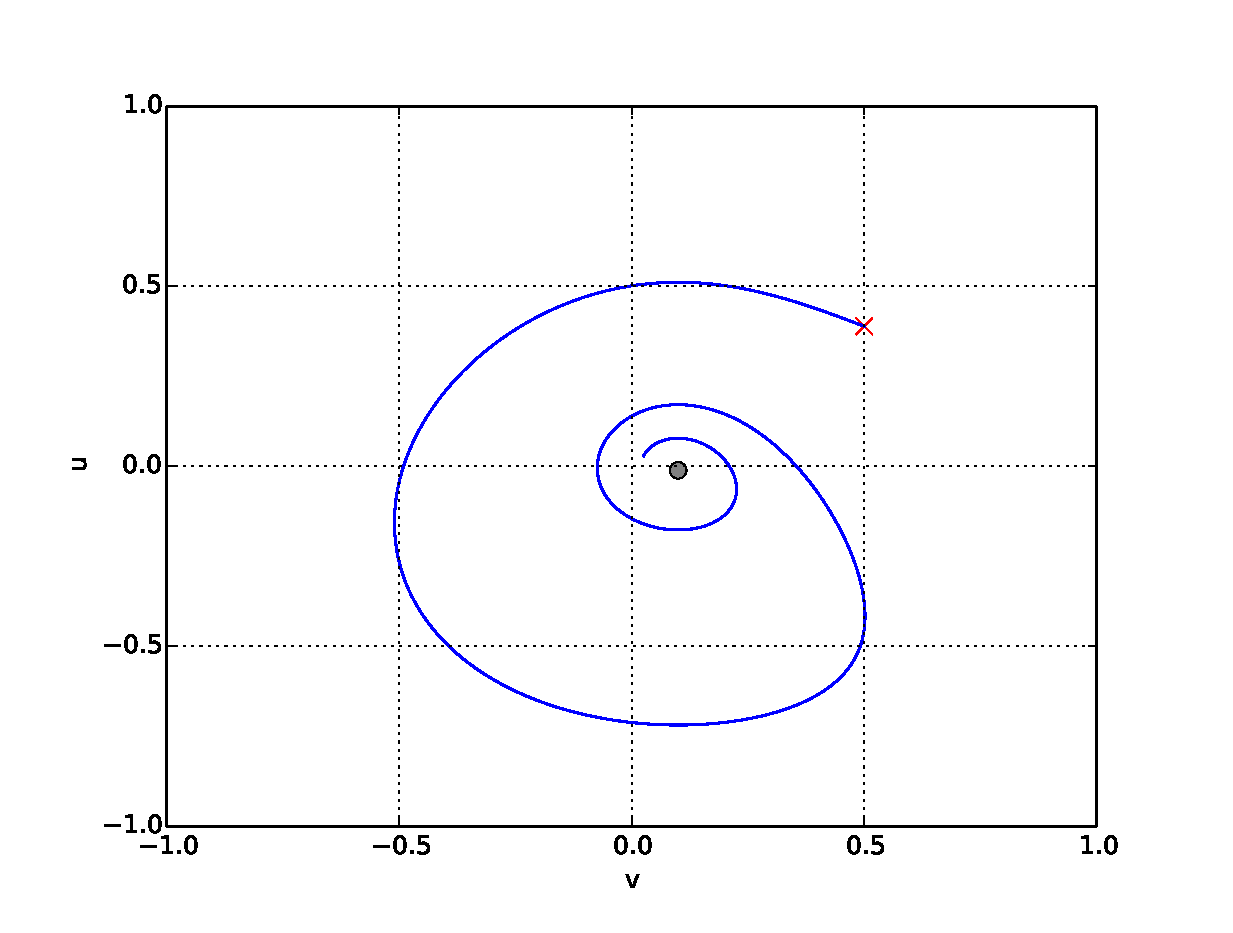
\includegraphics[width=5in]{../../andronovHopfGame/figures/phaseSpaceFirstRelaxationOscillatorSupercriticalBeforeLossOfStability.eps}
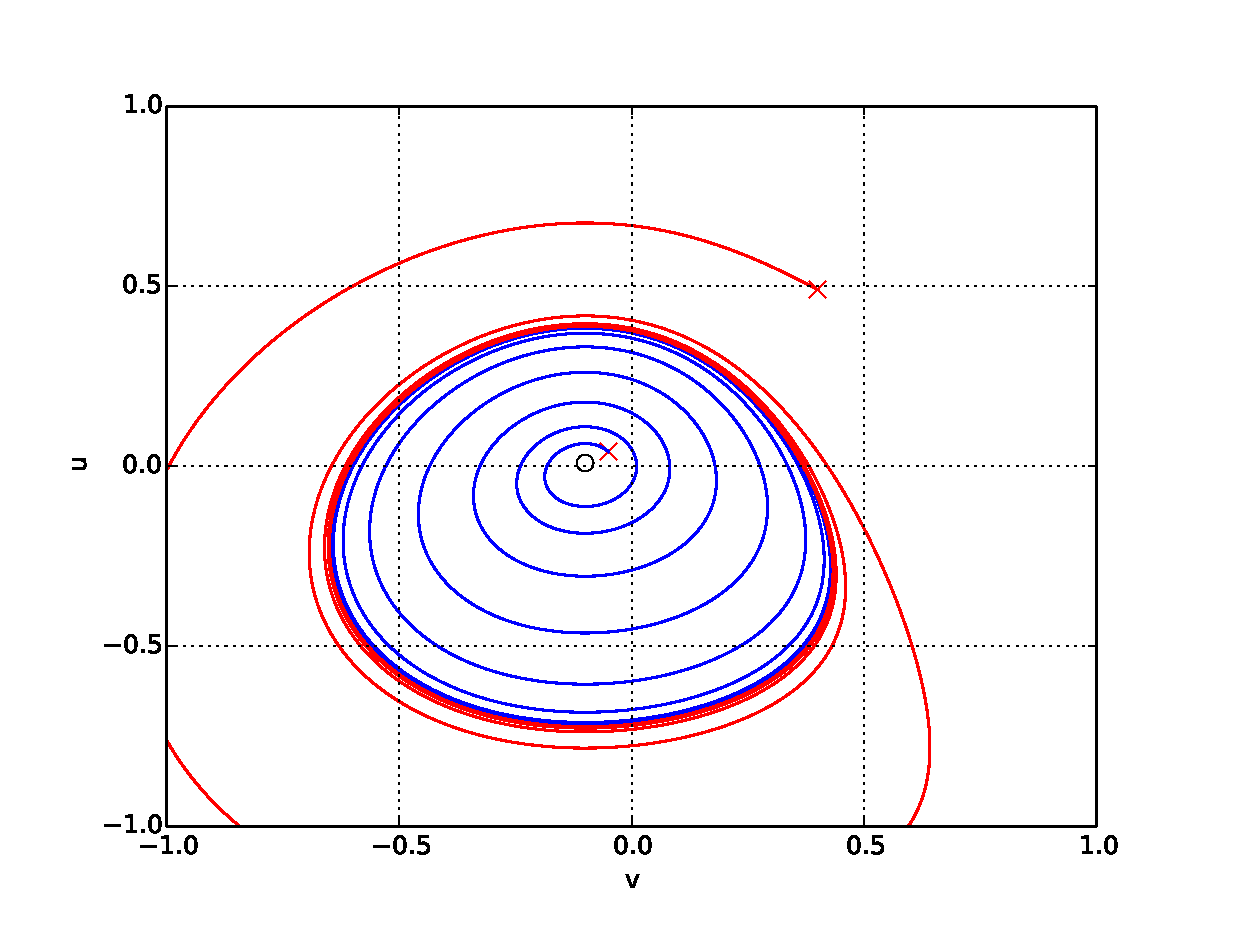
\includegraphics[width=5in]{../../andronovHopfGame/figures/phaseSpaceFirstRelaxationOscillatorSupercriticalAfterLossOfStability.eps}
\caption{Supercritical Andronov-Hopf bifurcation in the system in
Eq.~\ref{eq:system}.}
\label{fig:supercriticalAH}
\end{figure}
\end{center}

\section{Subcritical Andronov-Hopf Bifurcation}

Taking $f(v)=e^vv^2$ and $\mu=1$ in the system in Eq.~\ref{eq:system}
satisfies the above conditions for a subcritical Andronov-Hopf bifurcation.
Figure~\ref{fig:subcriticalAH} show trajectories of the system  in
Eq.~\ref{eq:system} with the above parameters before (b=-0.1, top panel in
Figure~\ref{fig:subcriticalAH}) and after (b=0.1, bottom panel
Figure~\ref{fig:subcriticalAH}) the unique equilibrium loses stability. As
expected for a subcritical Andronov-Hopf bifurcation as the equilibrium losses
stability an unstable limit cycle disappears.

\begin{center}
\begin{figure}
\includegraphics[width=5in]{../../andronovHopfGame/figures/phaseSpaceFirstRelaxationOscillatorSubcriticalBeforeLossOfStability.eps}
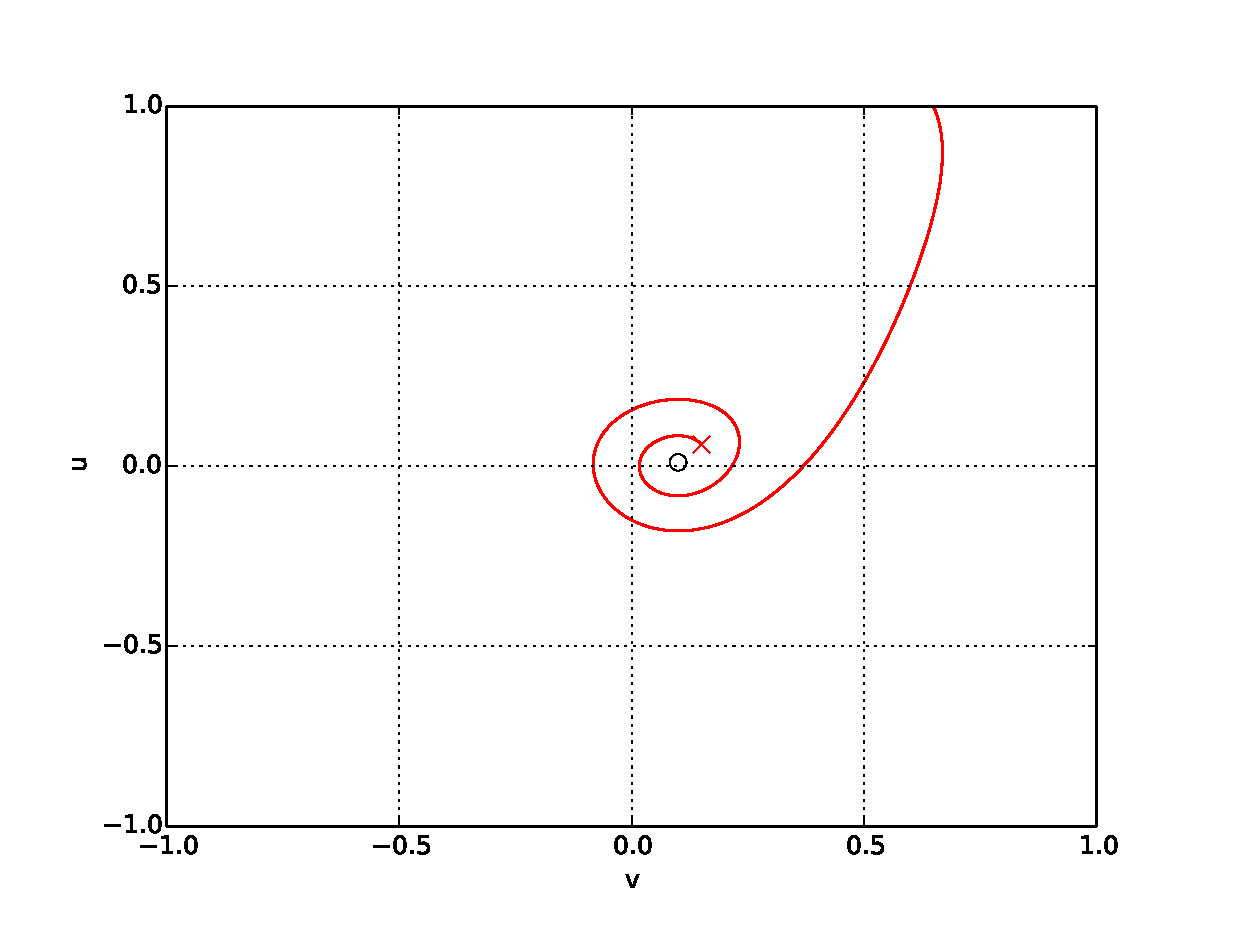
\includegraphics[width=5in]{../../andronovHopfGame/figures/phaseSpaceFirstRelaxationOscillatorSubcriticalAfterLossOfStability.eps}
\caption{Subcritical Andronov-Hopf bifurcation in the system in
Eq.~\ref{eq:system}.}
\label{fig:subcriticalAH}
\end{figure}
\end{center}

\bibliographystyle{apacite}
\bibliography{dynamicalSystems}

\end{document}
